\paragraph{高维情形。}\label{sub:high-dimensional-case}
设 $n\ge 2$。于是可以使用\cref{thm:functor-realization-obstruction}，再加上一个关于\trHochschildCohomology{}群的适当的消没结果，来证明任何以 $A^n_m$ 为\trCohomology{}的\trACategory{}都必然是形式的（即\trQuasiisomorphic{}于 $A^n_m$ 上的平凡\trAinfty{}结构——也就是使阶数 $>2$ 的\trComposition{}映射全都消没的那一个结构）。这在 [134] 中已经实现。在这里，我们对刚才提到的那个结果采取一种更具体的进路，以避开抽象的分类理论。在几何方面，它依赖于 §18 的内容，因而需要技术性假设 $\mathrm{char}(\KK)\ne 2$。
取函数 $\pi\colon X\to\CC$，$\pi(x)=x_0$。再经过一些技术调整之后，可以把 $\pi$ 视为一个\trLefschetzFibration，而把对 $(\Psi,\pi)$ 视为一个\trBifibration。此外，$\pi$ 的诸\trFiber{}与\trParallelTransport{}映射都可以得到显式的分析 [85]：每张\trSmooth\trFiber{}都\trSymplectic\trIsomorphic{}于\trCotangent{}丛 $T^*S^{n-1}$；每条\trVanishingPath{}都给出同一个\trVanishingCycle，即\trZeroSection{}$S^{n-1}\subset T^*S^{n-1}$；因此，每条连接两个\trCriticalValue{}的路径都平凡地是一条\trMatchingPath。特别地，诸 $V_j$ 便作为一列\trMatchingPath{}$\mu_j$（如\cref{fig:matching-cycles-chain}所示）的\trMatchingCycle{}而出现。
\begin{figure}[htbp]
\centering
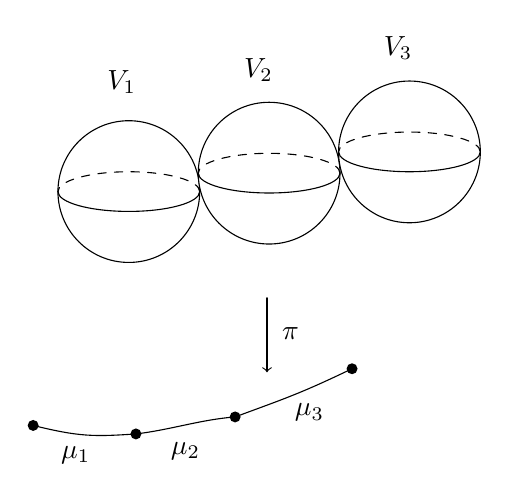
\begin{tikzpicture}[line cap=round,line join=round,scale=0.9]
\draw[fill=white] (0,0) circle (1.0);
\draw[dashed] (1.0,0) arc[x radius=1.0, y radius=0.28, start angle=0, end angle=180];
\draw (-1.0,0) arc[x radius=1.0, y radius=0.28, start angle=180, end angle=360];
\draw[fill=white] (1.98,0.26) circle (1.0);
\draw[dashed] (2.98,0.26) arc[x radius=1.0, y radius=0.28, start angle=0, end angle=180];
\draw (0.98,0.26) arc[x radius=1.0, y radius=0.28, start angle=180, end angle=360];
\draw[fill=white] (3.96,0.56) circle (1.0);
\draw[dashed] (4.96,0.56) arc[x radius=1.0, y radius=0.28, start angle=0, end angle=180];
\draw (2.96,0.56) arc[x radius=1.0, y radius=0.28, start angle=180, end angle=360];
\node at (-0.1,1.55) {$V_1$};
\node at (1.83,1.72) {$V_2$};
\node at (3.8,2.02) {$V_3$};
\draw[->] (1.95,-1.5) -- (1.95,-2.55);
\node at (2.28,-2.0) {$\pi$};
\fill (-1.35,-3.3) circle (2.2pt);
\fill (0.1,-3.42) circle (2.2pt);
\fill (1.5,-3.18) circle (2.2pt);
\fill (3.15,-2.5) circle (2.2pt);
\draw (-1.35,-3.3) .. controls (-0.7,-3.46) and (-0.5,-3.46) .. (0.1,-3.42);
\node at (-0.75,-3.72) {$\mu_1$};
\draw (0.1,-3.42) .. controls (0.6,-3.36) and (1.0,-3.22) .. (1.5,-3.18);
\node at (0.8,-3.66) {$\mu_2$};
\draw (1.5,-3.18) .. controls (2.2,-2.92) and (2.4,-2.86) .. (3.15,-2.5);
\node at (2.55,-3.12) {$\mu_3$};
\end{tikzpicture}
\caption{}\label{fig:matching-cycles-chain}
\end{figure}
从现在起固定 $m$ 与 $n\ge 2$，并记 $\scr{F}=\scr{F}^n_m$、$A=A^n_m$。如果只考虑位于其\trCotangent{}丛之内的\trZeroSection{}$S^{n-1}$，那么与之相伴的\trFukaya\trAinfty{}代数\trQuasiisomorphic{}于 $\KK\cdot e\oplus\KK\cdot f$，其中
\begin{equation}\label{eq:cotangent-aoo-algebra}
\begin{split}
&|e|=0,\ |f|=n-1,\\
&\mu^2(e,e)=e,\ \mu^2(e,f)=(-1)^{n-1}f,\ \mu^2(f,e)=f,
\end{split}
\end{equation}
而其余全部乘积均消没。这在\trCohomology{}的层面上是显然的，在那里我们看到的正是 $HF^*(S^{n-1},S^{n-1})=H^*(S^{n-1};\KK)$。在上链的层面上，必要的消没结果可由\trDegree{}方面的考虑推出，至少一旦把这个\trAinfty{}结构做成\trStrictlyUnital{}的便是如此（另一种办法是使用 [58] 的结果，以及 $S^{n-1}$ 在传统的代数\trTopology{}意义下是形式的这一事实）。下一步是写出与 $\pi$ 的\trVanishingCycle{}的一组基相伴的\trDirected\trAinfty\trCategory{}$\scr{B}^{\rightarrow}$，它当然就由 $S^{n-1}$ 的 $m+1$ 个副本组成。这是直截了当的：把诸\trObject{}记作 $(Z_0,\ldots,Z_m)$，则\trMorphism{}为
\begin{equation}\label{eq:directed-category-hom}
\hom_{\scr{B}^{\rightarrow}}(Z_i,Z_j)=
\begin{cases}
\KK\cdot e_{ji}\oplus\KK\cdot f_{ji}, & i<j,\\
\KK\cdot e_{ii}, & i=j,\\
0, & i>j,
\end{cases}
\end{equation}
其\trDegree{}与\trComposition{}一如 \eqref{eq:cotangent-aoo-algebra}。取 $Tw\scr{B}^{\rightarrow}$ 中由下式给出的诸\trObject{}$(C_1,\ldots,C_m)$：
\begin{equation}\label{eq:cone-objects}
C_j=\mathrm{Cone}(e_{j,j-1}).
\end{equation}
\cref{thm:matching-l-cone}说，由这些\trObject{}组成的\trFullSubcategory{}\trQuasiisomorphic{}于 $\scr{F}$。容易验证，在\trCohomology{}的层面上，这重新给出 $A$。更重要的是，这一过程给出了一个显式的链层面模型。最后，结果表明这个模型容许一个有用的附加对称性，而它\trApriori{}地并非来源于几何。
为简化记号，我们使用\cref{thm:shifted-multiplicity-spaces}的那个版本的\trTwistedComplex。给 $\scr{B}^{\rightarrow}$ 配备另一个按长度的\trGrading，使得诸 $e_{ji}$ 的长度为零，而诸 $f_{ji}$ 的长度为二（这个名字的理由将在后面说明）。于是可以引进\textbf{齐次\trAdditive\trCompletion{}}（homogeneous additive completion）$\Sigma^{\mathrm{ho}}\scr{B}^{\rightarrow}$，其\trObject{}是有限和
\begin{equation}\label{eq:homogeneous-completion}
\bigoplus_i S^{-\sigma_i}\Lambda^{-\tau_i}Y_i,
\end{equation}
其中 $\Lambda$ 是一个使长度\trGrading{}减一的形式运算。于是任何两个这样的\trObject{}之间的\trMorphism{}都带有一个按\trDegree{}与长度的双\trGrading。沿着同样的思路，我们有齐次\trTwistedComplex{}的\trAinfty\trCategory{}$Tw^{\mathrm{ho}}\scr{B}^{\rightarrow}$，其\trObject{}是表达式 \eqref{eq:homogeneous-completion} 连同一个保持长度\trGrading{}的\trDifferential。例如，\eqref{eq:cone-objects} 可以按如下方式变成一个齐次\trTwistedComplex：
\begin{equation*}
C_j=\Lambda^j\mathrm{Cone}(e_{j,j-1})=S\Lambda^j Z_{j-1}\oplus\Lambda^j Z_j,
\qquad
\delta_{C_j}=\begin{pmatrix}0 & 0\\ e_{j,j-1} & 0\end{pmatrix}.
\end{equation*}
一如之前，取 $Tw^{\mathrm{ho}}\scr{B}^{\rightarrow}$ 中由这些\trObject{}组成的\trFullSubcategory，它是一个双\trGraded{}\trAinfty\trCategory。在\trCohomology{}的层面上，这个附加的\trGrading{}确实重新给出 $A$ 作为 \eqref{eq:graded-quiver} 的\trPathAlgebra{}之\trQuotient{}所继承的那个长度\trGrading。
让我们把\cref{thm:perturbation-lemma}应用于前面构造的\trFullSubcategory，以消去 $\mu^1$。这可以按保持双\trGrading{}的方式来做，而结果便是 $A$ 上的一个对长度\trGrading{}齐次的\trAinfty{}结构 $\scr{A}$。细察表明，此时更高阶的\trComposition{}映射 $\mu^d_{\scr{A}}$（$d>2$）必然是平凡的。另一方面，我们的\trAinfty{}结构按构造\trQuasiisomorphic{}于 $\scr{F}$，故 $\scr{F}$ 是形式的。
